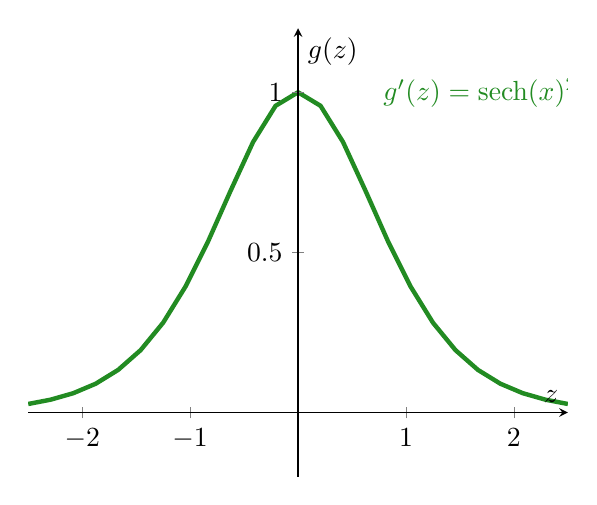
\begin{tikzpicture}
\begin{axis}[
    xmin=-2.5, xmax=2.5,
    ymin=-.2, ymax=1.2,
    axis lines=center,
    axis on top=true,
    domain=-2.5:2.5,
    ylabel=$g(z)$,
    xlabel=$z$,
    ]

    \addplot [mark=none,draw=ForestGreen,ultra thick] {4 / (exp(x) + exp(-x))^2};
    \node [right, ForestGreen] at (axis cs: 0.7,1) {$g'(z) = \textrm{sech} (x)^2$};
\end{axis}
\end{tikzpicture}